\documentclass[11pt,a4paper]{article}
\usepackage[margin=1in]{geometry}
\usepackage{graphicx}
\usepackage{booktabs}
\usepackage{amsmath,amssymb}
\usepackage{multirow}
\usepackage{hyperref}
\usepackage{xcolor}
\usepackage{float}
\usepackage{caption}
\usepackage{subcaption}

\definecolor{healthy}{RGB}{46,139,87}
\definecolor{warning}{RGB}{204,153,0}
\definecolor{danger}{RGB}{178,34,34}
\definecolor{notable}{RGB}{70,70,180}

\title{Experiment Report: \texttt{shakedown\_8b\_d1024\_k2}\\[0.3em]
\large Scale-Up Shakedown --- d=1024, 8 Blocks, k=2, 10K Steps}
\author{NL\_Hecate Research}
\date{March 16, 2026}

\begin{document}
\maketitle

\begin{abstract}
This report documents the \texttt{shakedown\_8b\_d1024\_k2} experiment: a scale-up of the
validated spec25 k=2 baseline from d=512/4-block to d=1024/8-block (55M $\to$ 118M parameters).
The run completes 10,000 steps on Dolmino-100B in 6.7 hours at 211 tok/s, achieving a final
loss of \textbf{3.37}. The primary finding is that the 8-block architecture develops
\textbf{extreme block-specific specialization} far beyond what the 4-block model exhibited:
Block~1 drives L0 alpha to 0.07 (near-zero retention), Block~2's L1 theta rises to 0.51
(active slow-level learning), and Blocks~4/7 partially shut their L0 output gates (eta $<$ 0.3).
The depth specialization CV reaches 0.84--0.92, compared to 0.34 at d=512. Notably, this run
omits the \texttt{alpha\_floor} constraint present in spec25, allowing the model to explore the
full gate parameter space. The run confirms that the segment-scoped tape supports d=1024 k=2
on a single A6000 without OOM.
\end{abstract}

\tableofcontents
\newpage

%=============================================================================
\section{Experiment Configuration}
%=============================================================================

\begin{table}[H]
\centering
\caption{Model and training configuration. Changes from spec25 baseline highlighted in bold.}
\begin{tabular}{llll}
\toprule
\textbf{Parameter} & \textbf{This Run} & \textbf{spec25 Baseline} & \textbf{Notes} \\
\midrule
\multicolumn{4}{l}{\textit{Architecture}} \\
\quad d\_model & \textbf{1024} & 512 & 2$\times$ \\
\quad num\_heads & \textbf{16} & 8 & 64-dim per head \\
\quad seq\_len & 512 & 512 & \\
\quad n\_blocks & \textbf{8} & 4 & 2$\times$ \\
\quad vocab\_size & 50,257 & 50,257 & \\
\quad params & \textbf{117,622,794} & 55,141,386 & $\sim$2.1$\times$ \\
\midrule
\multicolumn{4}{l}{\textit{CMS Configuration}} \\
\quad k (levels) & 2 & 2 & \\
\quad chunk\_sizes & [1, 8] & [1, 8] & \\
\quad memory\_rule & titans & titans & \\
\quad composition & mag & mag & \\
\quad parallel\_strategy & tnt\_hierarchical & tnt\_hierarchical & \\
\midrule
\multicolumn{4}{l}{\textit{Gate Constraints}} \\
\quad alpha\_floor & \textbf{None} & [0.8, 0.8] & Unconstrained \\
\quad theta\_ceil & [1.0, 1.0] & [1.0, 1.0] & \\
\quad m\_norm\_max & [100.0, 100.0] & [100.0, 100.0] & \\
\midrule
\multicolumn{4}{l}{\textit{Training}} \\
\quad steps & \textbf{10,000} & 30,000 & Shakedown length \\
\quad lr & 3e-4 & 3e-4 & \\
\quad warmup\_steps & 500 & 500 & \\
\quad optimizer & adamw\_gpu\_stacked & adamw\_gpu\_stacked & \\
\quad tape\_multiplier & 1 & 1 & Spec 25 \\
\quad save\_every & \textbf{500} & 5,000 & Dense checkpointing \\
\quad tape\_every & \textbf{500} & 1,000 & Finer tape sampling \\
\midrule
\multicolumn{4}{l}{\textit{Infrastructure}} \\
\quad GPU & 1$\times$ A6000 (48GB) & 1$\times$ A6000 (48GB) & \\
\quad data & Dolmino-100B & Dolmino-100B & \\
\bottomrule
\end{tabular}
\end{table}

\noindent Two intentional design differences from spec25:
\begin{enumerate}
    \item \textbf{No alpha\_floor}: The spec25 run constrained L0/L1 alpha $\geq$ 0.8. This run removes that floor, allowing the model to explore the full retention parameter space. This is the first run where alpha is fully unconstrained.
    \item \textbf{10K steps (shakedown length)}: The primary purpose is to validate that d=1024 k=2 runs stably on A6000 with the segment-scoped tape, and to observe what gate configurations emerge at scale. This is not a convergence run.
\end{enumerate}

%=============================================================================
\section{Results Summary}
%=============================================================================

\begin{table}[H]
\centering
\caption{Key metrics at training milestones.}
\begin{tabular}{rrrrrr}
\toprule
\textbf{Step} & \textbf{Loss} & \textbf{PPL} & \textbf{Grad Norm} & \textbf{Block CV} & \textbf{LR} \\
\midrule
0      & 10.895 & 53,886 & 22.06 & 0.369 & 0.00e+0 \\
500    &  5.157 &    174 &  2.24 & 0.847 & 3.0e-4 \\
1,000  &  4.770 &    118 &  3.09 & 1.190 & 3.0e-4 \\
2,000  &  4.074 &     59 &  2.76 & 1.176 & 2.9e-4 \\
5,000  &  4.732 &    114 &  3.56 & 1.030 & 1.5e-4 \\
7,000  &  3.591 &     36 &  2.70 & 0.999 & 6.6e-5 \\
10,000 &  3.371 &     29 &  2.11 & 0.835 & 8.2e-12 \\
\bottomrule
\end{tabular}
\end{table}

\begin{table}[H]
\centering
\caption{Scale-up comparison with spec25 baseline (first 10K steps).}
\begin{tabular}{lccc}
\toprule
\textbf{Metric} & \textbf{spec25 d=512 4b} & \textbf{shakedown d=1024 8b} & \textbf{Notes} \\
\midrule
Params & 55M & 118M & 2.1$\times$ \\
Loss @ 10K steps & $\sim$3.4 & 3.37 & Comparable \\
Throughput & 1,207 tok/s & 211 tok/s & 5.7$\times$ slower \\
Wall time (10K steps) & $\sim$1.2h & 6.7h & \\
Block CV (final) & 0.47 & \textbf{0.84} & 1.8$\times$ higher \\
Grad spikes ($>$10) & 2 (warmup) & 4 total & \\
Checkpoint size & 267 MB & \textbf{890 MB} & 3.3$\times$ \\
alpha\_floor & 0.8 & \textbf{None} & Key difference \\
\bottomrule
\end{tabular}
\end{table}

\noindent Key outcomes:
\begin{itemize}
    \item \textbf{Stability}: d=1024 k=2 runs cleanly on A6000 with segment-scoped tape. No OOM, no NaN. Only 2 non-warmup gradient spikes in 10K steps.
    \item \textbf{Loss}: 10.9 $\to$ 3.37 in 10K steps --- comparable to spec25 at the same step count despite 2$\times$ the model size. The model has ample capacity for longer training.
    \item \textbf{Block CV}: 0.84--0.92 throughout training --- dramatically higher than spec25's 0.34. The 8-block model develops extreme depth specialization that the 4-block model could not express.
    \item \textbf{Throughput}: 211 tok/s --- expected for 4$\times$ the FLOPS per token (d$^2$ scaling). The segment-scoped tape is not the bottleneck.
\end{itemize}

%=============================================================================
\section{Training Dynamics}
%=============================================================================

\subsection{Loss and Perplexity}

\begin{figure}[H]
\centering

\includegraphics[width=\textwidth]{loss_ppl.pdf}
\caption{Training loss and perplexity over 10K steps. Loss descends from 10.9 to $\sim$3.4 with healthy monotonic progress. The curve has not flattened --- significant headroom remains.}
\end{figure}

\subsection{Comparative Loss (d=512 vs d=1024)}

\begin{figure}[H]
\centering

\includegraphics[width=0.85\textwidth]{comparative_loss.pdf}
\caption{Loss comparison over the first 10K steps. Both models reach similar loss ($\sim$3.4) at 10K despite the 2$\times$ parameter difference. The d=1024 model's loss curve tracks slightly above the d=512 curve, consistent with larger models requiring more steps to exploit their capacity.}
\end{figure}

\subsection{Throughput}

\begin{figure}[H]
\centering

\includegraphics[width=0.85\textwidth]{throughput.pdf}
\caption{Training throughput. Mean 211 tok/s, stable throughout. The 5.7$\times$ reduction from spec25 (1,207 tok/s) is dominated by d$^2$ scaling of the memory operations and 2$\times$ the blocks.}
\end{figure}

\subsection{Learning Rate Schedule}

\begin{figure}[H]
\centering
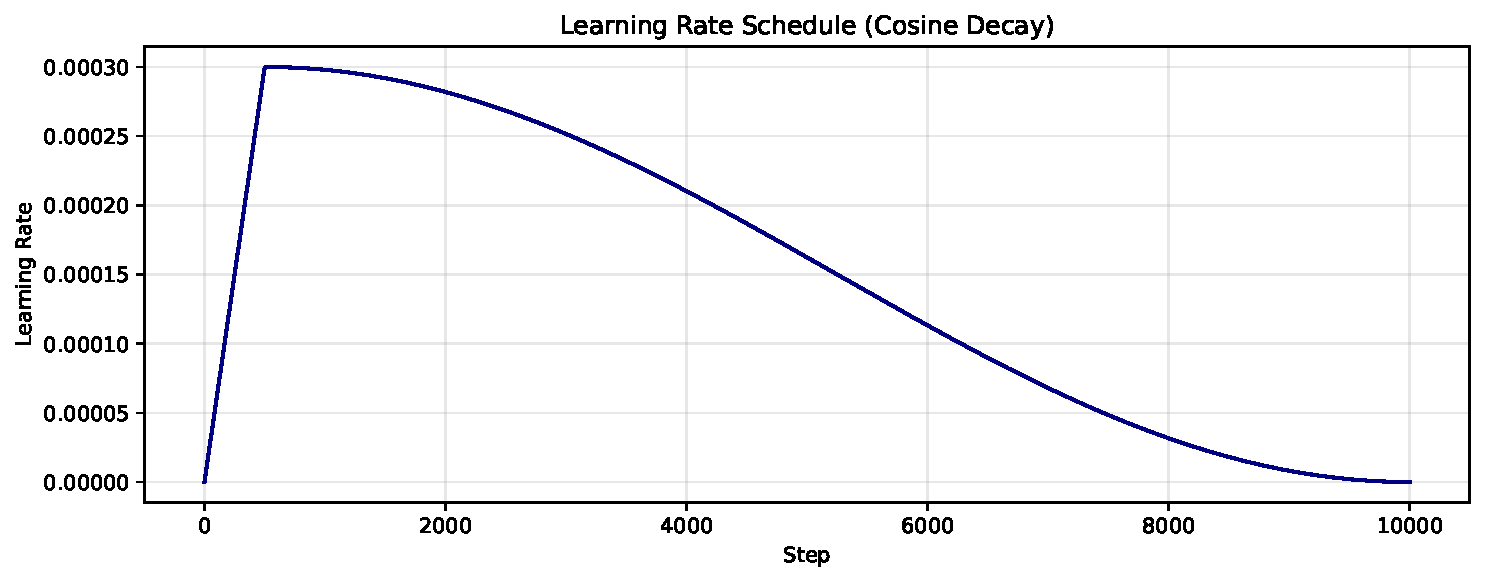
\includegraphics[width=0.85\textwidth]{lr_schedule.pdf}
\caption{Cosine decay learning rate schedule over 10K steps.}
\end{figure}

%=============================================================================
\section{Gradient Analysis}
%=============================================================================

\subsection{Global Gradient Norms and Depth Specialization}

\begin{figure}[H]
\centering

\includegraphics[width=\textwidth]{grad_norms.pdf}
\caption{Left: global gradient norm with 4 spike events marked. Right: block gradient norm CV. The CV is 0.84--1.2 throughout training --- far above the 0.3 threshold used for d=512. The d=512 baseline reference line (gray dashed) illustrates the scale difference.}
\end{figure}

The block CV of 0.84--1.2 is the most striking difference from the 4-block model. This means Block~0's gradient norm is \textbf{4--6$\times$ larger} than the interior blocks, indicating extreme input-adjacent specialization that 4 blocks simply cannot express.

\subsection{Per-Block Gradient Norms}

\begin{figure}[H]
\centering

\includegraphics[width=0.95\textwidth]{block_grad_norms.pdf}
\caption{Per-block gradient norms (8 blocks). Block~0 dominates at $\sim$0.8, while Blocks~1--7 cluster tightly around 0.15--0.20. This is a much sharper hierarchy than the 4-block model's gradual gradient taper.}
\end{figure}

\subsection{L0 Inner-Loop Gradient Signal}

\begin{figure}[H]
\centering

\includegraphics[width=0.95\textwidth]{l0_grad_norms.pdf}
\caption{L0 per-block gradient norms. Block~0 carries the largest L0 signal ($\sim$0.06--0.09), with notable variation across interior blocks --- Block~3 and Block~5 show periodic bursts.}
\end{figure}

%=============================================================================
\section{Gate Diagnostics: Block-Specific Specialization}
%=============================================================================

This section presents the central finding of the shakedown: the 8-block model develops
\textbf{dramatically different gate configurations per block}, far beyond the modest
block-to-block variation seen at d=512. The absence of \texttt{alpha\_floor} allows the
model to explore strategies that were previously clamped out.

\subsection{Gate Heatmap (Final Snapshot)}

\begin{figure}[H]
\centering
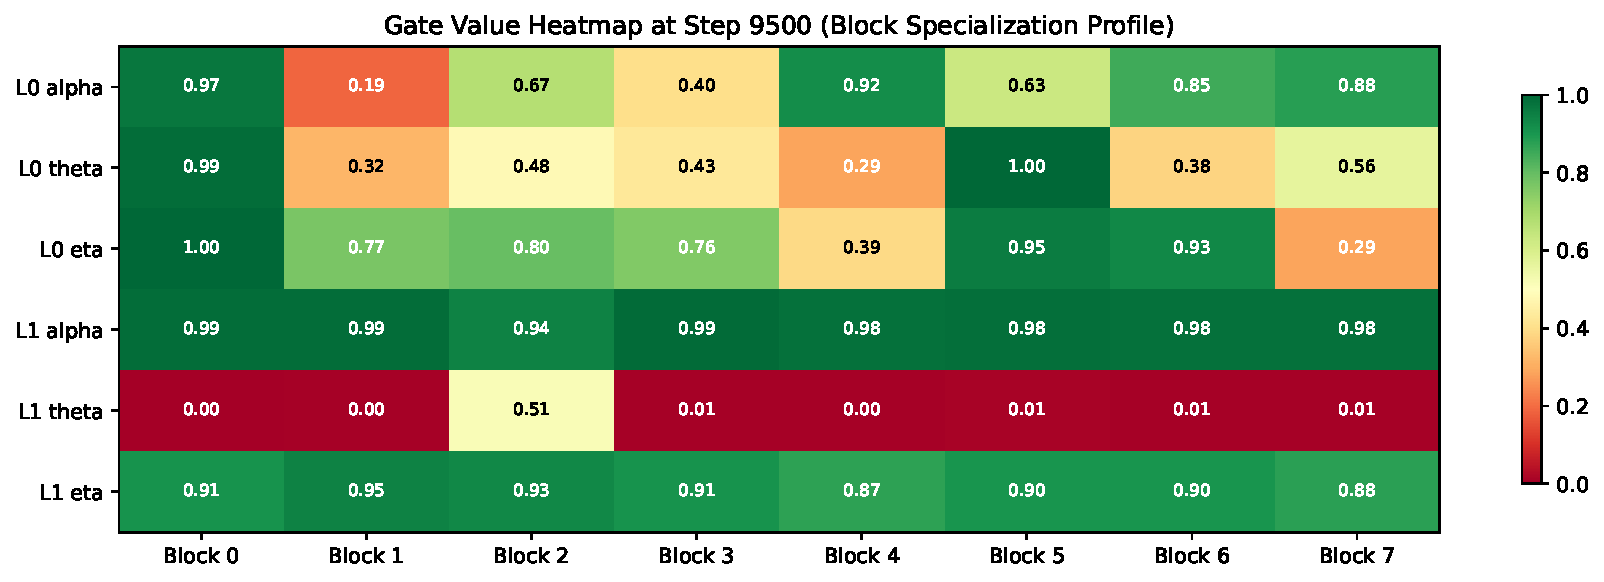
\includegraphics[width=0.95\textwidth]{gate_heatmap.pdf}
\caption{Gate values across all 8 blocks at step 9,500. Each cell shows the mean gate value for that block/level combination. The block-to-block variation in L0 alpha (0.19--0.99) and L0 eta (0.29--1.00) is the headline finding.}
\end{figure}

\noindent The heatmap reveals three distinct block archetypes:

\begin{table}[H]
\centering
\caption{Block archetype classification based on gate profiles.}
\small
\begin{tabular}{llp{8cm}}
\toprule
\textbf{Archetype} & \textbf{Blocks} & \textbf{Characteristics} \\
\midrule
\textbf{Stateless processor} & B1, B3 & L0 alpha $<$ 0.4 (near-zero retention), moderate theta. L0 acts as a pure transform --- reads memory, computes, but retains almost nothing. \\
\textbf{Gated specialist} & B4, B7 & L0 eta $<$ 0.4 (output gate nearly shut). L0 memory exists but is largely excluded from the output path. L1 dominates. \\
\textbf{Full engagement} & B0, B5, B6 & Both L0 and L1 active with high theta/eta. Classic dual-level CMS behavior matching the d=512 pattern. \\
\midrule
\textbf{Anomalous} & B2 & L1 theta = 0.51 --- the slow level is actively learning at near-L0 rates. L1 alpha = 0.94. This block has partially collapsed its frequency hierarchy. \\
\bottomrule
\end{tabular}
\end{table}

\subsection{Theta (Inner-Loop Learning Rate)}

\begin{figure}[H]
\centering

\includegraphics[width=\textwidth]{theta_evolution.pdf}
\caption{Theta evolution: L0 (top row) vs L1 (bottom row) across all 8 blocks. L0 theta shows much more block-to-block variation than at d=512 --- Block~0 saturates to 1.0, while Blocks~1,3,6 settle around 0.3--0.5. L1 theta stays near zero in all blocks except Block~2, where it rises to 0.51 by step 3,500 and holds.}
\end{figure}

\noindent\textbf{Block 2 L1 theta anomaly}: Block~2's L1 theta rises from 0.004 to 0.51 between steps 3,000--3,500. This means L1 is performing memory updates at half the rate of L0 --- far faster than the ``slow level'' should operate. The L1 alpha simultaneously drops from 0.98 to 0.94, reducing its retention advantage. Block~2 has partially collapsed the fast/slow distinction. This is the first time L1 theta has broken 0.1 in any run.

\subsection{Alpha (Retention Gate) --- Unconstrained}

\begin{figure}[H]
\centering

\includegraphics[width=\textwidth]{alpha_evolution.pdf}
\caption{Alpha evolution: L0 (top row, full 0--1 scale) vs L1 (bottom row, 0.85--1.0 scale). Without alpha\_floor, L0 alpha spans the entire range: Block~0 stays near 0.97, Block~1 drops to 0.07, Blocks~3,5 oscillate around 0.2--0.6. L1 alpha remains high ($>$0.94) across all blocks.}
\end{figure}

\noindent\textbf{The unconstrained alpha finding}: Removing alpha\_floor reveals that the model \textit{wants} very different retention strategies per block:
\begin{itemize}
    \item \textbf{Block 0}: L0 alpha $\sim$0.97 --- the input-adjacent block retains heavily, similar to the alpha\_floor=0.8 regime. The floor was not binding here.
    \item \textbf{Block 1}: L0 alpha oscillates 0.07--0.35 --- near-zero retention. This block treats L0 memory as disposable, rewriting it almost completely each step. A fundamentally different strategy from Block~0.
    \item \textbf{Block 9 (B9 = B1)}: The 0.07 minimum at step 9,000 is the lowest alpha observed in any NL-Hecate run. The alpha\_floor of 0.8 in spec25 would have completely prevented this behavior.
    \item \textbf{L1 alpha}: Stays $>$0.94 everywhere. Even unconstrained, the slow level maintains high retention. This validates the alpha\_floor design --- it was never binding for L1.
\end{itemize}

\subsection{Eta (Output Gate)}

\begin{figure}[H]
\centering

\includegraphics[width=\textwidth]{eta_evolution.pdf}
\caption{Eta evolution: L0 (top row) vs L1 (bottom row). Blocks~4 and 7 progressively shut their L0 output gates to $\sim$0.3, while L1 eta remains high ($>$0.87) across all blocks. The model is learning to selectively suppress L0 contributions at specific depths.}
\end{figure}

\noindent The L0 eta suppression in Blocks~4/7 is architecturally significant: the model is using the MAG gating mechanism to create \textit{L1-dominant} blocks at specific depths while maintaining dual-level blocks elsewhere. This is depth-dependent frequency selection --- something the 4-block model with alpha\_floor could not express.

\subsection{DGD Ratio (L0/L1 Update Magnitude)}

\begin{figure}[H]
\centering
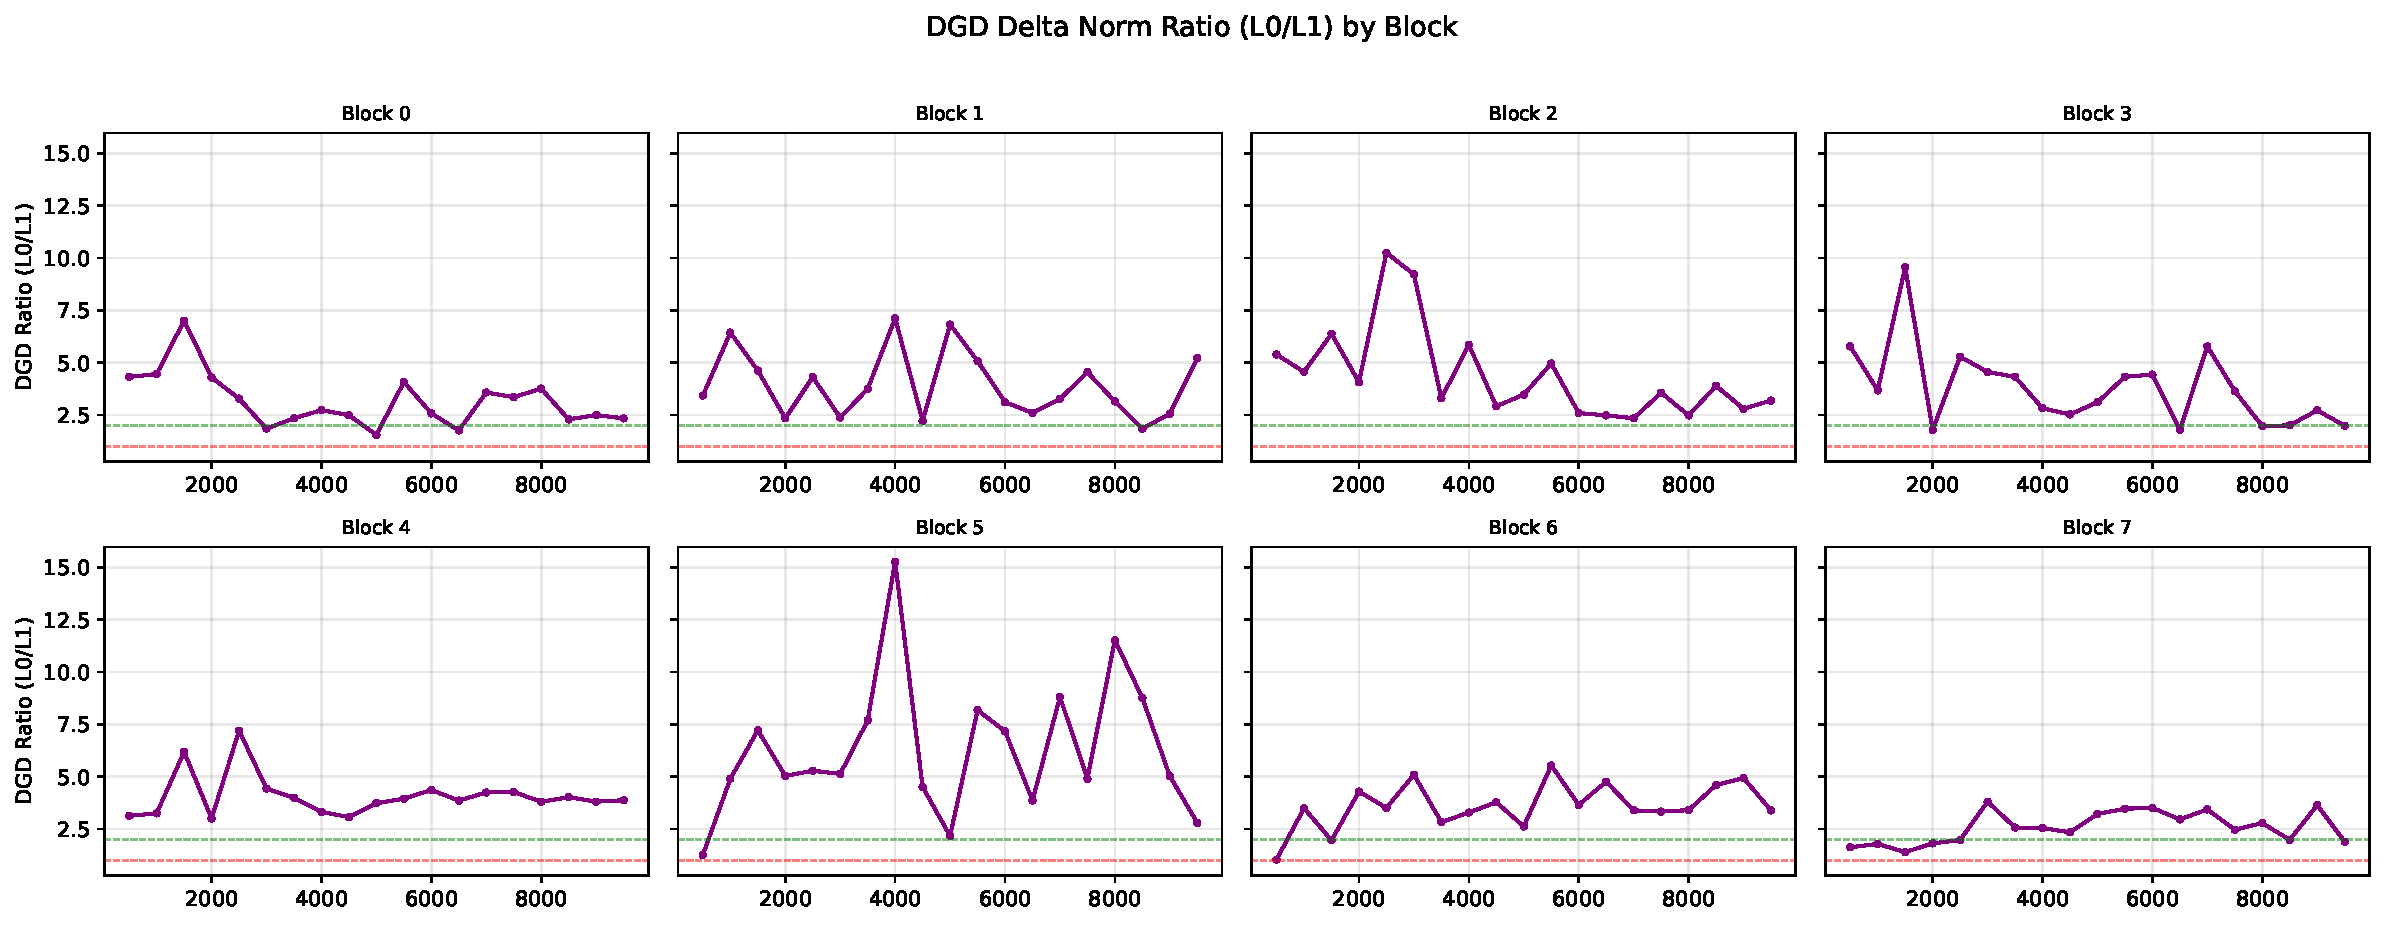
\includegraphics[width=\textwidth]{dgd_ratio.pdf}
\caption{DGD delta norm ratio (L0/L1) across 8 blocks. Most blocks maintain healthy ratios of 2--5$\times$, with Block~0 peaking at 7$\times$. The ratios are consistently above the 2.0 threshold (green dashed), with occasional transient dips.}
\end{figure}

\subsection{Output Gradient Norms (MAG Identity Check)}

\begin{figure}[H]
\centering
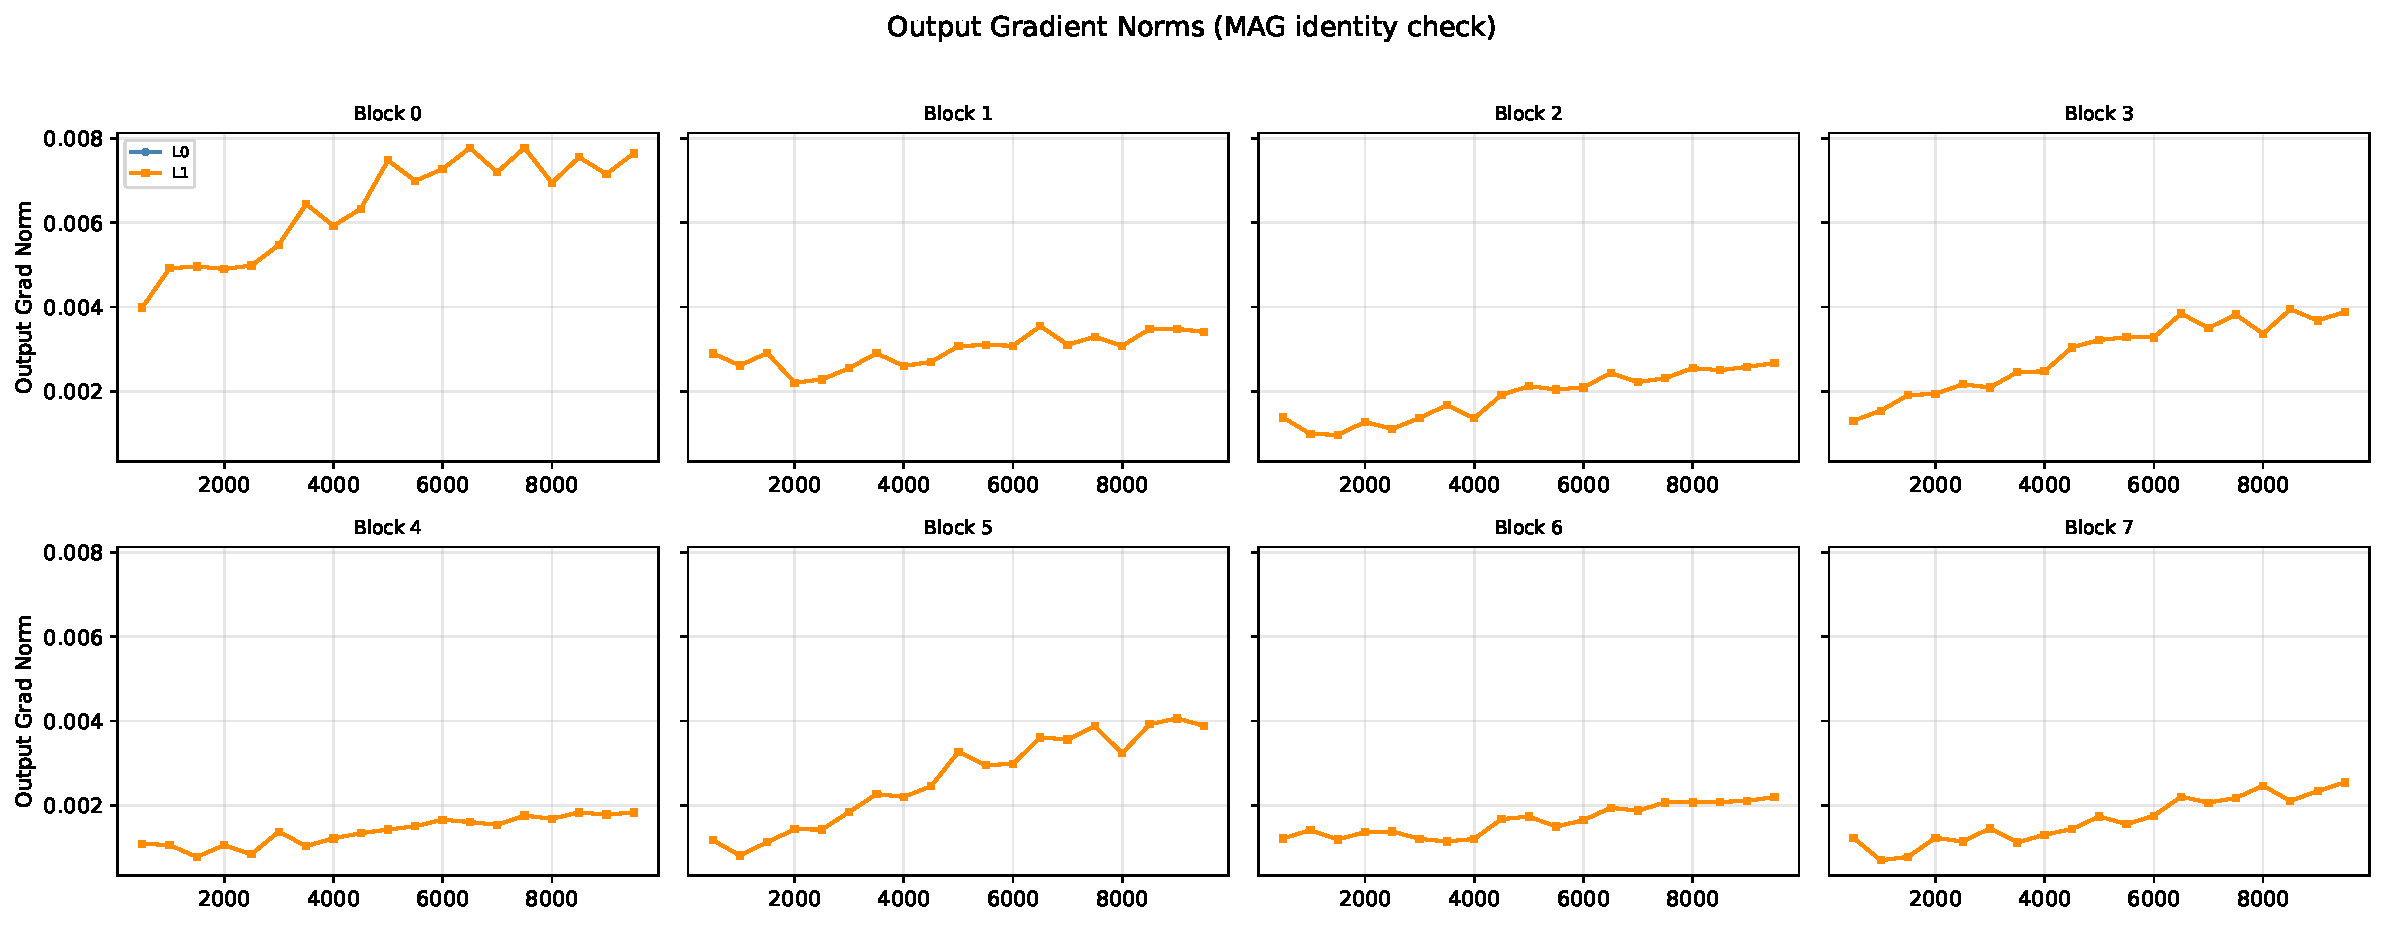
\includegraphics[width=\textwidth]{output_grad_norms.pdf}
\caption{Output gradient norms: L0 and L1 overlap perfectly in all blocks, confirming the MAG structural identity holds at d=1024/8-block.}
\end{figure}

%=============================================================================
\section{Scale-Up Analysis}
%=============================================================================

\subsection{What Scales Cleanly}

\begin{itemize}
    \item \textbf{Loss trajectory}: Comparable loss at 10K steps despite 2$\times$ parameters. The larger model is not overparameterized for this task at this step count.
    \item \textbf{Stability}: Zero NaN, only 4 gradient spikes (2 in warmup). The segment-scoped tape handles d=1024 without modification.
    \item \textbf{L1 behavior}: L1 theta stays near zero, L1 alpha stays high ($>$0.94), DGD ratios are healthy. The slow level's behavior scales cleanly from 4 to 8 blocks.
    \item \textbf{MAG identity}: Output gradient identity holds across all 8 blocks.
\end{itemize}

\subsection{What Changes at Scale}

\begin{itemize}
    \item \textbf{Block CV}: 0.34 $\to$ 0.84--0.92. The 8-block model develops extreme depth specialization. Block~0 carries 4--6$\times$ the gradient load of interior blocks.
    \item \textbf{Block specialization}: The 4-block model showed modest block-to-block gate variation. The 8-block model develops three distinct block archetypes (stateless, gated, full). This is qualitatively new behavior.
    \item \textbf{Unconstrained alpha}: Without alpha\_floor, L0 alpha spans the full 0.07--0.99 range per block. The model wants block-specific retention strategies that the floor would prevent.
    \item \textbf{Block 2 anomaly}: L1 theta = 0.51 is unprecedented. At 8 blocks, the model has enough depth to ``sacrifice'' one block's frequency hierarchy for a different optimization strategy.
\end{itemize}

\subsection{Implications for alpha\_floor}

The unconstrained alpha results suggest that alpha\_floor=0.8 may be overly conservative for deep models:
\begin{itemize}
    \item Block~0 naturally stays above 0.8 even without the floor --- the constraint was not binding.
    \item Blocks~1,3 drive alpha well below 0.8, suggesting the floor was suppressing a useful optimization strategy at those depths.
    \item The floor may need to be \textbf{per-block} rather than global, or removed entirely and replaced with a softer regularization.
    \item However, this is a 10K shakedown --- the low-alpha strategy may not survive a longer training run. A 30K+ run without alpha\_floor is needed to confirm.
\end{itemize}

%=============================================================================
\section{Conclusions}
%=============================================================================

The shakedown validates three things:

\begin{enumerate}
    \item \textbf{Infrastructure}: The segment-scoped tape (Spec~25) supports d=1024 k=2 on a single A6000 with stable throughput ($\sim$211 tok/s) and no OOM. The path to d=1024 k=4 via Spec~27 (per-level tape strategy) is clear.

    \item \textbf{Depth specialization}: 8 blocks produce qualitatively different behavior from 4 blocks. The model develops block-specific archetypes (stateless, gated, full engagement) that were invisible at smaller scale. This is not merely ``more of the same'' --- it is a phase transition in architectural expressivity.

    \item \textbf{Unconstrained gates}: Removing alpha\_floor reveals that the model wants dramatically different retention strategies per block. This finding should inform the alpha\_floor decision for production k=4 runs: either remove it, make it per-block, or use it only as a stability floor during early training and anneal it to zero.
\end{enumerate}

\subsection{Open Questions}

\begin{itemize}
    \item \textbf{Block 2 anomaly}: Is L1 theta = 0.51 a transient artifact of the short run, or does it persist? If it persists, Block~2 has effectively merged its frequency hierarchy --- the 8$\times$ ratio between L0 and L1 no longer holds at that depth.
    \item \textbf{Alpha floor vs. no floor}: Does the near-zero L0 alpha in Blocks~1,3 help or hurt at 30K+ steps? It may be an early-training artifact that causes instability later.
    \item \textbf{Throughput}: 211 tok/s is 5.7$\times$ slower than d=512. For production k=4 at d=1024, Spec~27 must deliver not just memory savings but also throughput improvements from reduced backward-pass computation on proxy levels.
\end{itemize}

\subsection{Next Steps}

\begin{enumerate}
    \item \textbf{Spec 27 implementation}: Per-level tape strategy --- currently in progress. Required for k=4 at d=1024.
    \item \textbf{Replicate on Spec 27}: Re-run this shakedown config on the Spec~27 codebase to validate the per-level tape at d=1024.
    \item \textbf{Extended d=1024 run}: 30K steps with and without alpha\_floor to determine whether the block specialization patterns persist or are early-training transients.
    \item \textbf{k=4 shakedown}: Once Spec~27 is implemented, d=1024 k=4 8-block to validate VRAM fits within A6000 budget ($\sim$4.6 GB tape).
\end{enumerate}

\end{document}
